\chapter{Referencial Teórico}\label{cap:referencial_teorico}

\section{Twitter}\label{sec:twitter}

Contando com uma base ativa de usuários que ultrapassa 300 milhões\cite{twittercompany2016}, o Twitter é conhecido como um \emph{microblog} fundado em março de 2006 por Jack Dorsey, Evan Williams e Biz Stone. Após 10 anos de mercado, a empresa acumula números impressionantes: 300 bilhões de mensagens já foram compartilhadas por seus usuários, que em média enviam 500 milhões de \emph{tweets}\cite{twitterstats2016} - nome pelo qual as mensagens ficaram conhecidas na internet - por dia. Os usuários trocam mensagens de até 140 caracteres\cite{twittercharlimit2016} em um ambiente de rede social, que tem como objetivo dar à todos o poder de criar e compartilhar ideias e informações instantaneamente, sem barreiras\cite{twittercompany2016}. 

Dentro do Twitter, O usuário pode fazer uso de marcadores conhecidos como \emph{hashtags}\cite{waite2012paperback}, para vincular sua mensagem à um tópico específico. Apesar de simples, as \emph{hashtags} pode ser usadas das mais diversas maneiras:
\begin{itemize}
\item Agrupar comentários e pensamentos acerca de um tema
\item Estabelecer uma conexão entre dois tópicos
\item Aproximar o usuários de um conteúdo relevante com auxílio de uma busca
\end{itemize}

\subsection{Primavera Árabe}
Um dos exemplos mais recentes e impressionantes de como as redes sociais desempenharam o papel de aproximar ideologias semelhantes e encorajar debates sociais profundos foi a Primavera Árabe - onda de manifestações e protestos que tiveram início em dezembro de 2010, tendo como cenário o Norte da África e Oriente Médio. Os principais alvos foram os regimes ditatoriais e patriarcais que há muito tempo estavam no poder.\cite{howard2011opening}. Redes sociais foram amplamente utilizadas para marcar encontros, debates e manifestações, além de mostrar para o mundo o que acontecia em tempo real, através do Twitter e outras redes sociais, como o YouTube.

\begin{figure}[ht]
	
	\centering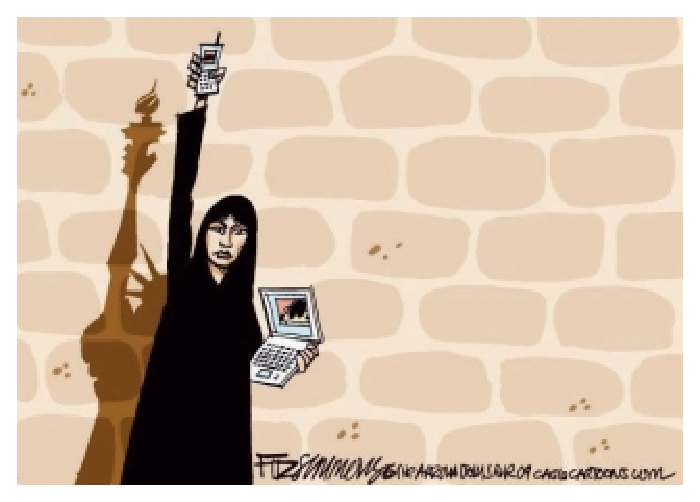
\epsfig{file=figuras/primavera_arabe_redes_sociais.eps, width=10cm}
	\caption{O celular e a internet foram as armas dos rebeldes na Primavera Árabe}
	\label{uni}
\end{figure}

\subsection{Análises de redes sociais}
Este novo cenário possibilitou que a análise de redes sociais ganhasse incrível relevância nos campos de pesquisa social e comportamental\cite{wasserman1994advances}. Ao invés de analisar comportamentos individuais, atitudes e crenças, a análise de redes sociais foca sua atenção em entidades sociais ou atores interagindo entre si e como essas interações constituem uma estrutura que pode ser estudada e analisada.

Outro ponto levantado recorrentemente quando o assunto é análise de redes sociais é o como ela pode ser útil para estudos de ordem \textit{micro} ou \textit{macro}. No nível \textit{micro}, as análises destinam-se a examinar díades, tríades ou outros pequenos sub-grupos. No nível \textit{macro}, o objeto de estudo são grandes redes de atores sociais.
Todos os dados obtidos durante a coleta permitem segmentar os atores sociais de diversas formas - gênero, idade, religião, posição demográfica, entre outros - possibilitando análises \textit{micro} - a nível de apenas um usuário - ou \textit{macro} - quando analisamos um conjunto de usuários. Por exemplo, os dados extraídos a partir da API do Twitter, que será abordada no Capítulo 3, nos permite entender como um usuário específico reagiu a uma \textit{hashtag}. Da mesma forma, podemos olhar um cenário mais amplo, como por exemplo, todos usuários de uma região do país. As possibilidades de análise crescem e se tornam mais ricas conforme obtemos mais informações sobre os atores no momento de suas interações sociais.

\section{Mineração de opinião}\label{sec:mineracao_dados}

* O que é?* Exemplos no mercado* Etapas(http://www.inf.ufsc.br/~alvares/INE5644/MineracaoOpiniao.pdf)

É de conhecimento comum que há um acúmulo de dados por toda a internet. Artigos, informações de usuários, comportamento de usuários, essas são alguns tipos de informação que pode ser encontrada hoje na internet. Esse grande acumulo não garante informações confiáveis ou uma análise correta sobre os dados, por isso hoje há uma grande urgência para novas teorias computacionais e ferramentas que ajudem a analisar essa quantidade de dados que só aumenta \cite{fayyad1996data}. E dentro dessa enorme gama de dados, existem as informações adicionadas por usuários através de texto que remetem a suas reações a determinadas situações ou objetos.

\begin{figure}[ht]
	\centering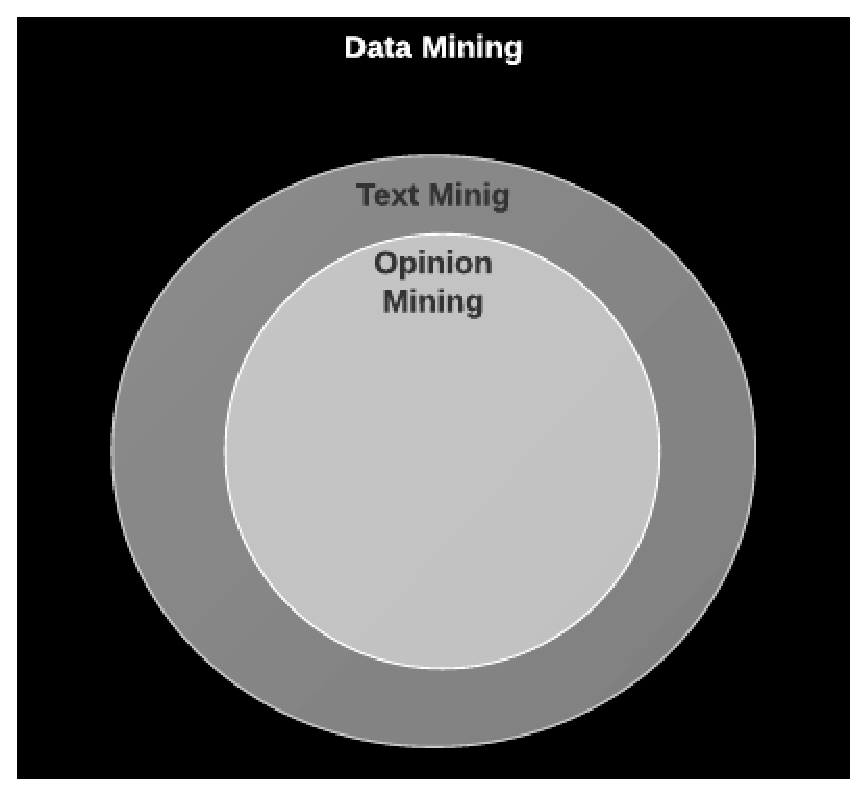
\epsfig{file=figuras/venn.eps, width=5cm}
	\caption{Diagrama de Venn - Mineração de Dados}
	\label{uni}
\end{figure}


\subsection{Definição}
A mineração de opinião também conhecida como mineração de sentimento, análise de sentimento ou extração de opinião, é um campo dentro da mineração de dados \cite{santos2014mineraccao}. Ela tem como intuito extrair o sentimento do texto escrito por uma pessoa, sem a interferência humana durante o processo. Existe dificuldade em afirmar o que é sentimento, na maioria dos dicionários sentimento é:
\begin{itemize}
\item Ato ou efeito de sentir.
\item Aptidão para receber as impressões.
\item Sensação; sensibilidade.
\item Consciência íntima.
\item Faculdade de compreender; intuição; percepção.
\end{itemize}

Porém de acordo com psicólogo Klaus R. Scherer, sentimento é um breve episódio da resposta sincronizada de todos os ou grande parte dos subsistemas orgânicos em resposta a um evento interno ou externo de grande significância. \cite{scherer2001emotional}

\section{API}\label{sec:api}
* O que é
* APIs mais utilizadas no mundo (case do twitter)
* Papel de uma API para integração de serviços (achar referência foda)

\section{Processamento de linguagem natural}\label{sec:nlp}
* Linguagem natural (foto da matéria de autômato do Aquino?)
* Processamento de linguagem natural
* Dificuldades dentro da nossa área de estudo


\section{Naive Bayes}\label{sec:naive_bayes}
* O que é o Naive Bayes
* Demonstração matemática do algoritmo
* Uso dele em analise de sentimento/classificação


\emph{Naive Bayes} é um algoritmo probabilístico. Baseado no teorema de bayes. $$ P(A \mid B) = \frac{P(B \mid A) \, P(A)}{P(B)} $$ onde se infere qual é a probabilidade de um evento A dado um evento B. Porém nesse trabalho é utilizado o \emph{Naive Bayes} e sua diferença para o teorema de Bayes é assumir que a posição das palavras que aparecem no texto não importa, daí é acrescentado o \emph{naive}(ingênuo) ao teorema.
\\ Como visto em \cite{lucca2013implementaccao} o algoritmo computa qual a probabilidade de uma frase, denominada de documento pertencer a uma determinada classe(polaridade) \emph{P(c/d)}, a partir da probabilidade a \emph{priori} de \emph{P(c)} do documento pertencer a esta classe e da probabilidades condicionais de cada termo \emph{tk} ocorrer em um documento da mesma classe. O algoritmo tem como objetivo encontrar a melhor classe para um documento maximizando a probabilidade a\emph{posteriori} conforme a equação abaixo, onde $ n_{d} $ é o número de termos no documento \emph{d}. $$ C_{map}= argmax_{c \epsilon C}P(c|d)=argmax_{c \epsilon C}P(c)\prod 1sksn_{d}P(t_{k}/d) $$